\documentclass{beamer}

\title{Summer 2025}
\author{Aatu Selkee}
\date{August 21, 2025}


\usepackage{subfigure}

\begin{document}

\frame{\titlepage}


\begin{frame}{Main research topics}
    \textbf{Time series analysis with Gaussian processes:}
    \begin{itemize}
        \item How to represent a difficult time series with a Gaussian processes
        \begin{itemize}
            \item Trend + Periodicity (daily, weekly, monthly, yearly) + Peaks + Noise
        \end{itemize}
        \item Choose the correct covariance function to model these effects.
        \item How to scale model training to 50 000 training points.
        \item How to improve the performance of Gaussian processes with a new feature representation from deep learning.
    \end{itemize}
\end{frame}

\begin{frame}{Gaussian processes}
    \begin{figure}
        \centering
        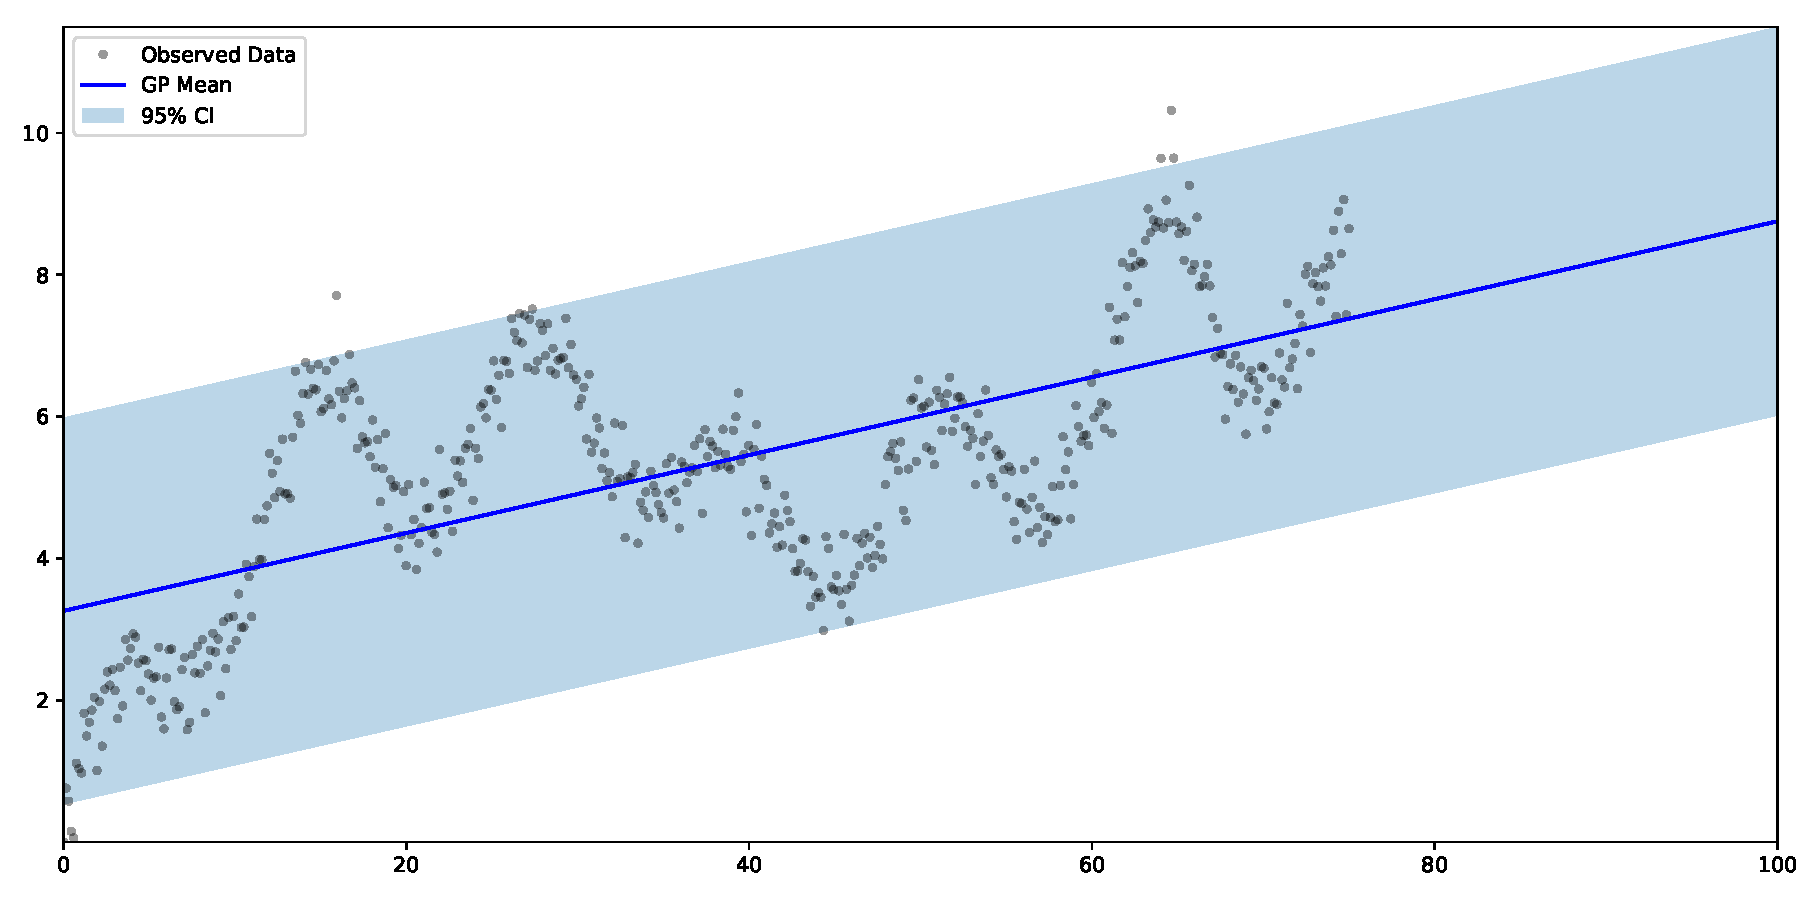
\includegraphics[width=\textwidth]{../Images/EndOfSummerPresentation/TSPredDemoLinear.pdf}
        \caption{The model captures the linear trend.}
    \end{figure}
\end{frame}

\begin{frame}{Gaussian processes}
    \begin{figure}
        \centering
        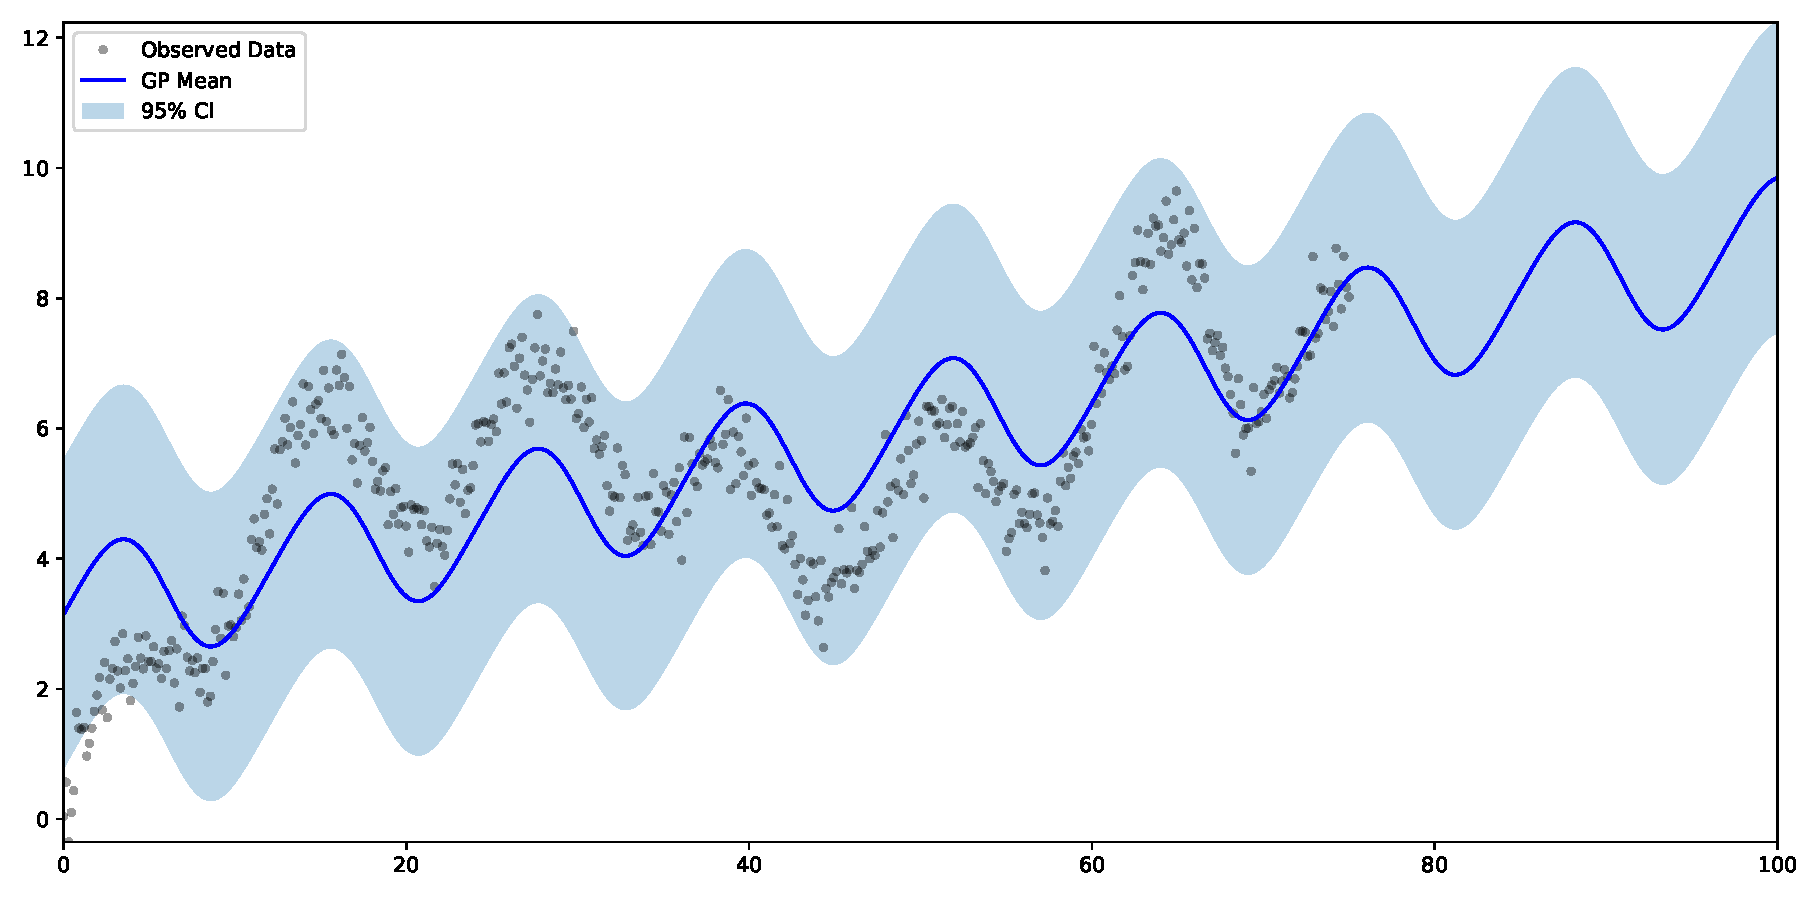
\includegraphics[width=\textwidth]{../Images/EndOfSummerPresentation/TSPredDemoLinearPeriodic.pdf}
        \caption{The model captures the linear trend and the periodicity.}
    \end{figure}
\end{frame}

\begin{frame}{Gaussian processes}
    \begin{figure}
        \centering
        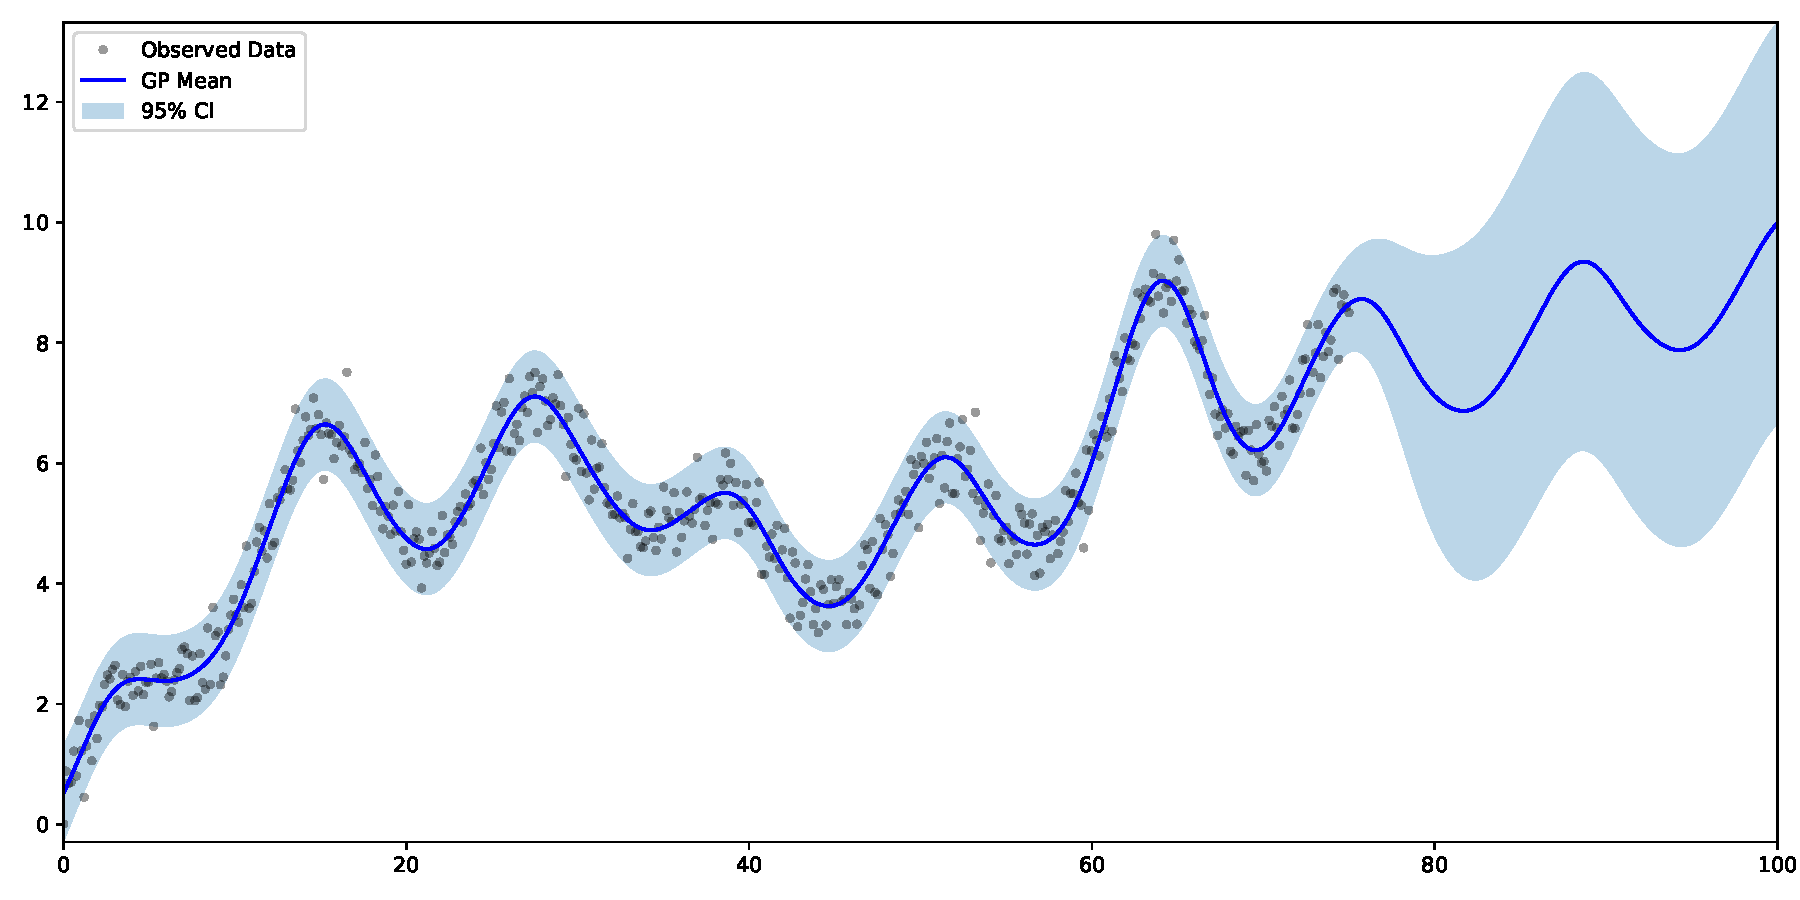
\includegraphics[width=\textwidth]{../Images/EndOfSummerPresentation/TSPredDemoLinearPeriodicRBF.pdf}
        \caption{The model captures the linear trend, the periodicity and the varying peaks. Only random noise is impossible to model.}
    \end{figure}
\end{frame}

\end{document}